\section{The oracle ladder}
\label{app:oracles}

\begin{table}[h]
\centering
\caption{Schedule-pooled relative score error of the two oracles against the tree-exact
reference, 512 chains per family at the frozen configuration. The LMMSE column is the
floor of every second-order estimator (\cref{prop:lmmse}).}
\begin{tabular}{lccc}
\toprule
family & excess kurtosis & isotropic $-\vx$ & LMMSE, true $\Sig_0$ \\
\midrule
Laplace & $+3$ & \isoFloorLaplace & \lmmseFloorLaplace \\
Student-$t_5$ & $+6$ & \isoFloorStudent & \lmmseFloorStudent \\
uniform & $-1.2$ & \isoFloorUniform & \lmmseFloorUniform \\
bimodal & $-0.72$ & \isoFloorBimodal & \lmmseFloorBimodal \\
Gaussian & $0$ & \isoFloorGaussian & \lmmseFloorGaussian \\
\bottomrule
\end{tabular}
\end{table}

\section{The second-order floor across correlation}
\label{app:phase}
The frozen configuration fixes $\corr=0.85$. The price of second-order closure is a function
of $\corr$ as well as of the innovation law, and this appendix reports it over
$\corr\in\{0,0.3,0.6,0.85,0.95\}$ for five families on the twelve-level schedule, computed
from the exact score with no estimation involved.
The heavy-tailed family is quoted from a recomputation on the
$(\phaseWideN,\phaseWideA)$ domain (\textsc{e07c}): on the operating grid the quadrature
sweep of \cref{app:numerics} places its $\corr=0$ cell outside the validated envelope, one
to two sites per bundle lying beyond the domain and pinned to its boundary. Widening the
domain moves its pooled floor by at most $\phaseStudentMoveOperating$ from $(801,8)$ to
$(801,12)$ and by at most $\phaseStudentMoveWide$ from $(801,12)$ to
$(\phaseWideN,\phaseWideA)$ (\textsc{e07b}, \textsc{e07c}), and every other family by at
most $\phaseOtherMoveWide$ between the operating and the widest grid; the other families
are quoted from the operating grid, where they are converged.
\IfFileExists{sections/phase-numbers.tex}{%% Included by 05-experiments.tex only when sections/phase-numbers.tex exists (E07 done).
\begin{figure}[t]
  \centering
  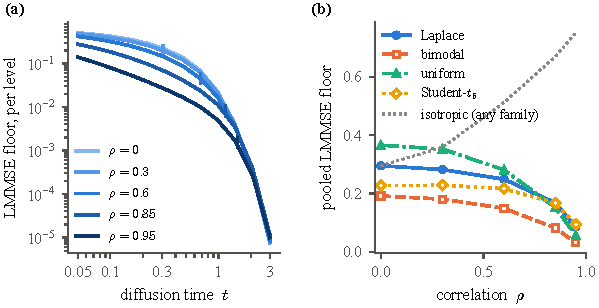
\includegraphics[width=\columnwidth]{fig_phase.pdf}
  \caption{\textbf{The second-order floor across correlation.} (a)~Per-level LMMSE
  floor on the Laplace chain for five $\corr$ (ticks: $\tstar(\corr)$); the floor
  collapses after the crossover. (b)~Schedule-pooled floor against $\corr$ for four
  innovation families, with the isotropic reference: strong correlation makes the score
  energy second-order-dominated, so the relative price of closure falls with $\corr$ while
  the absolute fourth-order structure does not.}
  \label{fig:phase}
\end{figure}
\paragraph{Across correlation.}
The floor is a function of the innovation law and of $\corr$ (\cref{fig:phase}): on the
Laplace chain it is $\phaseLmmseLaplaceRhozero$ for independent sites, $\phaseLmmseLaplaceRhozeropeightfive$
at the frozen $\corr=0.85$ and $\phaseLmmseLaplaceRhozeropninefive$ at $\corr=0.95$, where
$\tstar=\phaseTstarRhozeropninefive$ and the covariance carries most of the score energy
until late in the schedule. The families order by the size of their fourth cumulant at
every $\corr$; the isotropic reference rises with $\corr$ because the covariance itself is
what an unstructured estimator must learn first.
}{}

\section{Capacity: the previous reading, and why it is void}
\label{app:capacity}
An earlier study of this model compared innovation mixtures of $\ncomp\in\{1,2,4,8,16\}$
at $\nseq\in\{128,512\}$ over sixteen seeds and concluded that no capacity improved on a
single Gaussian innovation, attributing the estimator's margin over the networks to the
Markov factorisation and its covariance alone. That sweep is void for a reason prior to
any reading of it: its training draw re-created the random generator for every sequence,
so every arm at every capacity and seed was fitted to a single chain of $\nsites$ sites
(its validation and test bundles were drawn correctly). The signature is in its own
numbers: \cref{prop:lmmse} places a correctly fitted $\ncomp=1$ kernel on the LMMSE floor,
$\lmmseFloorLaplace$ on the Laplace chain, where \cref{sec:experiments} and all fifteen
cells of the regime sweep land to $\regIdentMax$, and the earlier sweep's single-Gaussian
arm scatters across a range several times wider. The stopping asymmetry that sweep also
shows (its likelihood tolerance fired for almost every single-Gaussian cell and for no
cell with $\ncomp\ge4$, so that the richer arms reported checkpoints far past their
optimum) is the behaviour of \textsc{em} on one chain, not evidence about capacity in
either direction; we had first read it as the explanation of the earlier conclusion, and
withdraw that reading. The capacity experiment of \cref{sec:experiments} draws every
chain independently, asserts it, and selects the checkpoint identically for every
capacity on a per-seed validation bundle; the same defect was found and fixed in one of
our own drivers before any of its numbers reached a page (\cref{app:protocol}).

\section{Capacity across the innovation family}
\label{app:family}
\IfFileExists{sections/family-numbers.tex}{%% Included by 05-experiments.tex only when sections/family-numbers.tex exists (E02b done).
\begin{figure}[t]
  \centering
  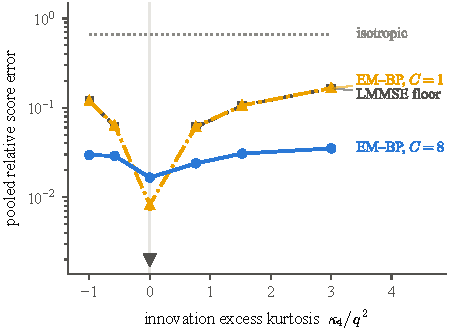
\includegraphics[width=\columnwidth]{fig_family.pdf}
  \caption{\textbf{Capacity buys exactly what the closure discards.} Pooled relative score
  error against the innovation's excess kurtosis for the generalised-Gaussian family at
  fixed $\corr$ and variance ($\nseq=\famSize$, $\famSeeds$ seeds, $\pm$ s.e.): the
  Gaussian-innovation kernel tracks the LMMSE floor, which is the exact price of
  second-order closure for each member; the mixture kernel tracks the exact score, and
  the two meet at the Gaussian member, where there is nothing beyond second order to
  learn.}
  \label{fig:family}
\end{figure}
Moving the innovation from Laplace (excess kurtosis $+3$) through the Gaussian to the
platykurtic end at fixed covariance (\cref{fig:family}), the LMMSE floor falls from
$\famLmmseBone$ to zero at $\beta=2$ and rises again to $\famLmmseBsix$; the
Gaussian-innovation kernel follows it, and the mixture kernel stays near
$\famEmeightBone$--$\famEmeightBsix$ throughout. The paired gain of $\ncomp=8$ over
$\ncomp=1$ is $\famDiffBone$ ($[\famDiffBonelo,\famDiffBonehi]$) at the Laplace end and
$\famDiffBtwo$ ($[\famDiffBtwolo,\famDiffBtwohi]$) at the Gaussian member, where the
two kernels are the same estimator up to sampling noise. Non-Gaussian capacity is worth
what \cref{thm:decay} says it is worth: the fourth-order structure the covariance twin
leaves behind.
}{\needsdata{E02b queued}}

\section{The capacity contrast across regimes}
\label{app:regimes}
\IfFileExists{sections/regime-numbers.tex}{%% Included by 05-experiments.tex only when sections/regime-numbers.tex exists (E13 done).
The capacity result above is measured at one point of the model's parameter space, so we
re-ran the contrast that carries it across $\regCells$ regimes: correlations from
$\regRhoLo$ to $\regRhoHi$ and chain lengths from $\regLenLo$ to $\regLenHi$, everything
else at the frozen protocol, $\regSeeds$ seeds each. The mixture beats the Gaussian
kernel in $\regAllExcludeZero$ cells with the paired interval excluding zero, by
$\regGainStrongest$ at the most favourable corner and $\regGainWeakest$ at the least.
The sweep also checks the apparatus at every point rather than only at the frozen
configuration: \cref{prop:lmmse} says the $\ncomp=1$ arm must coincide with the LMMSE of
the true covariance, and it does, to $\regIdentMax$ in the worst of the $\regCells$
cells, with a fitted excess kurtosis of at most $\regFitKurtOneMax$ in absolute value.
The $\ncomp=8$ arm recovers the innovation's true excess kurtosis of $3$ everywhere
($\regFitKurtLo$ to $\regFitKurtHi$ across correlations), and its spread widens from
$\pm\regFitKurtSdLo$ to $\pm\regFitKurtSdHi$ as $\corr$ rises---the shape becomes harder
to see, not differently placed.

The advantage itself shrinks monotonically with $\corr$, which is the direction
\cref{sec:theory} gives: a strongly correlated chain has a nearly Gaussian marginal, its
excess kurtosis falling as $3(1-\corr^2)/(1+\corr^2)$ from $\regKurtHi$ at
$\corr=\regRhoLo$ to $\regKurtLo$ at $\corr=\regRhoHi$, so there is less fourth-order
structure for capacity to buy. We report this as a direction and not as a rate: the
pooled error runs over a schedule whose informative window moves with $\corr$, so its
trend is not the exponent of \cref{thm:gap} and we do not fit one to it.
}{\needsdata{E13 pending}}

\section{Generation and length extrapolation: the tables}
\label{app:tables}
\IfFileExists{sections/generation-numbers.tex}{%% GENERATED by tools/make_generation_numbers.py from outputs/E05 -- do not hand-edit.
\begin{table}[t]\centering\small\setlength{\tabcolsep}{4pt}
\caption{Generated samples against the true law at $t_{\min}$: mean log-likelihood gap $\Delta\ell$ to the reference sample under the true $P_{t_{\min}}$ (exact evidence; the exact arm's gap is the sampler's discretisation floor), innovation excess kurtosis $\hat\kappa_4$, lag fourth cumulant, sliced $W_2$; the row marked \emph{reference} carries the reference sample's own statistics. Mean over seeds.}
\label{tab:generation}
\begin{tabular}{@{}llrrrr@{}}
\toprule
$\nseq$ & arm & $\Delta\ell$ & $\hat\kappa_4$ & lag-$\kappa_4$ & $W_2$ \\
\midrule
128 & \emph{reference} & -- & 1.94 & 0.000 & -- \\
 & exact & 0.074 & 1.86 & 0.000 & 0.051 \\
 & em--bp & 0.204 & 1.68 & 0.000 & 0.078 \\
 & lmmse & 1.761 & 0.00 & 0.000 & 0.053 \\
 & isotropic & 46.241 & 0.00 & 0.006 & 0.244 \\
 & net:bigru & 0.752 & 1.10 & 0.006 & 0.160 \\
 & net:window & 1.284 & 1.27 & 0.004 & 0.154 \\
\midrule
2048 & \emph{reference} & -- & 1.94 & 0.000 & -- \\
 & exact & 0.070 & 1.87 & 0.000 & 0.051 \\
 & em--bp & 0.164 & 1.80 & 0.001 & 0.055 \\
 & lmmse & 1.766 & 0.00 & 0.000 & 0.053 \\
 & isotropic & 46.295 & 0.00 & 0.010 & 0.244 \\
 & net:bigru & 0.385 & 1.55 & 0.003 & 0.167 \\
 & net:window & 1.115 & 1.46 & 0.003 & 0.139 \\
\bottomrule
\end{tabular}
\end{table}
}{}
\IfFileExists{sections/baseline-numbers.tex}{%% GENERATED by tools/make_baseline_numbers.py -- do not hand-edit.
\begin{table}[t]\centering\small\setlength{\tabcolsep}{4pt}
\caption{Length extrapolation at $\nseq=2048$: pooled relative score error of estimators fitted at $\nsites=32$ and evaluated against the tree-exact score of longer chains, mean over $\baseSeeds$ seeds. Longer chains are slightly easier (proportionally fewer boundary sites), so a length-agnostic arm should improve a little; the transformer instead breaks down beyond its training length.}
\label{tab:length}
\begin{tabular}{@{}lcccc@{}}
\toprule
arm & $\nsites=32$ & $\nsites=64$ & $\nsites=128$ & $\nsites=256$ \\
\midrule
bi-GRU & 0.060 & 0.057 & 0.057 & 0.056 \\
EM--BP & 0.023 & 0.023 & 0.023 & 0.023 \\
TCN & 0.068 & 0.066 & 0.065 & 0.064 \\
transf. & 0.063 & 0.243 & 0.514 & 0.703 \\
U-Net & 0.066 & 0.064 & 0.062 & 0.062 \\
window & 0.118 & 0.099 & 0.088 & 0.082 \\
\bottomrule
\end{tabular}
\end{table}
}{}
